\documentclass{article}
\usepackage{arxiv}

\usepackage[utf8]{inputenc}
\usepackage[english, russian]{babel}
\usepackage[T1]{fontenc}
\usepackage{url}
\usepackage{booktabs}
\usepackage{amsfonts}
\usepackage{nicefrac}
\usepackage{microtype}
\usepackage{bm}
\usepackage{lipsum}
\usepackage{graphicx}
\usepackage{natbib}
\usepackage{doi}
\usepackage{mathtools}


\newcommand{\argmin}{\arg\!\min}
\newcommand{\argmax}{\arg\!\max}


\title{Автоматическая регуляризации байесовских нейронных сетей}

\author{
    Басов Дмитрий Константинович
}
\date{}

\renewcommand{\shorttitle}{Автоматическая регуляризации байесовских нейронных сетей}
\numberwithin{equation}{section}

\begin{document}
    \maketitle

    \begin{abstract}
        В байесовском выводе, в отличии от гипотезы максимального правдоподобия,
        не делается никаких предположений о размере обучающей выборки.
        Это делает байесовские модели устойчивыми к переобучению.

        Однако применение байесовского вывода сопряжено со следующими проблемами:
        заданием подходящего априорного распределения и вычислением апостериорного распределения весов модели.

        В данной работе предлагается следующее решение этих проблем:
        \begin{enumerate}
            \item Применяя вариационный вывод,
                апостериорное распределение весов модели аппроксимируется
                нормальным распределением с диагональной матрицей ковариации,
                и задача сводится к максимизации нижней вариационной границы.
                В этом случае каждый вес модели определяется двумя обучаемыми параметрами.
            \item Априорное распределение весов модели задается в виде
                нормального распределения с нулевым матожиданием
                и диагональной матрицей ковариации, элементы которой вычисляется из данных.
                Этот приём лежит в основе Relevance Vector Machine~--- байесовского варианта SVM.
        \end{enumerate}

        Полученную модель можно рассматривать как
        ансамбль из бесконечного числа нейронных сетей,
        веса которых сэмплируются из нормального распределения.
        При этом каждый вес имеет свой индивидуальный коэффициент $L2$ регуляризации,
        который автоматически определяется из тренировочных данных при обучении.

    \end{abstract}

    \section{Обозначения и сокращения}
    $\pmb{x} \odot \pmb{y}$ --- поэлементное произведение (произведение Адамара) векторов \par
    $\mathcal{L}$ --- Evidence Lower Bound (ELBO) \par
    $
        KL(q~||~p)
        =
        \int_{}{
            q(\pmb{Z})
            \,
            \ln{
                \frac
                    {q(\pmb{Z})}
                    {p(\pmb{Z})}
            }
            \,
            d\pmb{Z}
        }
    $ --- дивергенция Кульбака--Лейблера (KL--дивергенции) \par
    $\pmb{x}$ --- вектор признаков \par
    $\pmb{y}$ --- вектор целевой переменной \par
    $D$ --- датасет --- пары значений $\{\pmb{x_i}$, $\pmb{y_i}\}$, где $i = 1, \dots, L$ \par
    $\pmb{W}$ --- веса модели --- случайная величина размерности M \par
    $p(\pmb{y} | \pmb{x}, D)$ --- предсказательное распределение \par
    $
        p(D | \pmb{W})
        =
        \prod_{i=1}^{L}{
            p(\pmb{y_i} | \pmb{x_i}, \pmb{W})
        }
    $ — правдоподобие (likelihood) \par
    $p(\pmb{W})$ --- априорное распределение весов модели (prior) \par
    $p(\pmb{W}| D)$ --- апостериорное распределение весов модели (posterior) \par
    $q_{\pmb{\theta}}(\pmb{W})$ --- аппроксимация апостериорного распределения весов модели \par
    $\pmb{\theta}$ --- обучаемые параметры байесовской модели \par

    \section{Введение}

    В классическом машинном обучении делается следующее предположение:
    веса модели $\pmb{W}$ являются пусть и неизвестной, но фиксированной величиной.
    В этом случае можно получить точечную оценку весов модели согласно гипотезе максимального правдоподобия:
    \begin{equation}
        \pmb{W_{ML}} = \argmax_{\pmb{W}} p(D | \pmb{W})
    \end{equation}
    Тогда распределение $p(\pmb{y} | \pmb{x}, D)$ аппроксимируется следующим образом:
    \begin{equation}
        p(\pmb{y} | \pmb{x}, D) \approx p(\pmb{y} | \pmb{x}, \pmb{W_{ML}})
    \end{equation}
    Однако это справедливо при условии, что количество объектов в датасете D
    сильно больше количества весов модели ($L \gg M$).
    Если это не так, веса модели $\pmb{W}$ могут слишком сильно подстроиться
    под обучающую выборку D, что черевато переобучением.

    Для борьбы с переобучением используется ряд приёмов (штрафы на норму весов, early stopping, dropout),
    однако для их настройки требуются вычислительные ресурсы и отложенные
    (не участвующие в обучении) выборки данных.

    Альтернативным подходом к машинному обучению является нахождение апостериорного распределения весов модели $p(\pmb{W}| D)$ по теореме Байеса.
    \begin{equation}
        p(\pmb{W}| D)
        =
        \frac
            {
                p(D | \pmb{W})
                \,
                p(\pmb{W})
            }
            {
                \int_{}{
                    p(D | \pmb{W})
                    \,
                    p(\pmb{W})
                    \,
                    d\pmb{W}
                }
            }
    \end{equation}
    Тогда предсказательное распределение $p(\pmb{y} | \pmb{x}, D)$ рассчитывается следующим образом:
    \begin{equation}
        p(\pmb{y} | \pmb{x}, D)
        =
        \int_{}{
            p(\pmb{y} | \pmb{x}, \pmb{W})
            \,
            p(\pmb{W} | D)
            \,
            d\pmb{W}
        }
    \end{equation}
    Байесовские модели можно рассматривать как ансамбль из бесконечного числа моделей,
    веса которых сэмплируются из распределения
    $p(\pmb{W}| D)$.
    Такой подход устойчив к переобучению, так как о размере обучающей выборки не делается никаких предположений.
    Однако возникают следующие проблемы: выбор подходящего априорного распределения
    $p(\pmb{W})$
    и вычисление апостериорного распределения
    $p(\pmb{W}| D)$.

    Неудачный выбор $p(\pmb{W})$ может сильно ухудшить качество модели,
    а расчёт апостериорного распределения $p(\pmb{W}| D)$
    требует вычисления интеграла по всему пространству весов модели,
    что для нейронных сетей практически невозможно.

    В данной статье предлагается следующий подход к решению этих проблем.

    \begin{enumerate}
        \item Применяя вариационный вывод, распределение $p(\pmb{W}| D)$
            аппроксимируется распределением $q_{\pmb{\theta}}(\pmb{W})$,
            и задача сводится к максимизации нижней вариационной границы
            $\mathcal{L}$ по параметрам $\pmb{\theta}$.
        \item Распределение $q_{\pmb{\theta}}(\pmb{W})$
            задаётся в виде нормального распределения с диагональной матрицей ковариации.
%             То есть каждый вес модели определяется двумя числами,
%             которые определяют его математическое ожидание и дисперсию.
%             Таким образом, количество обучаемых параметров
%             относительно классической нейронной сети возрастает в 2 раза.
        \item Так как распределение $q_{\pmb{\theta}}(\pmb{W})$
            является нормальным, применяя трюк с репараметризацией,
            становится возможным использовать градиентные методы
            для максимизации $\mathcal{L}$.
        \item Априорное распределение весов модели $p(\pmb{W})$
            задаётся в виде нормального распределения с нулевым матожиданием
            и диагональной матрицей ковариации, элементы которой определяются при обучении из датасета D.
            Такой подход обладает большой универсальностью,
            однако из--за этого теряется теоретическая устойчивость к переобучению.
            Идея определения некоторых параметров априорного распределения
            $p(\pmb{W})$ из датасета D
            известна как эмпирический Байес.
        \item Вводятся новые параметры $\pmb{\gamma}$ и $\pmb{\rho}$,
            через которые выражаются матожидание и дисперсия распределения
            $q_{\pmb{\theta}}(\pmb{W})$.
            Это нужно, чтобы избежать неопределенности деления $\frac{0}{0}$,
            которая может возникнуть из--за определения дисперсии распределения $p(\pmb{W})$ из данных.
    \end{enumerate}

    \section{Постановка задачи}

    Задача машинного обучения с учителем
    в вероятностной постановке формулируется следующим образом: получить
    распределение вероятностей $p(\pmb{y} | \pmb{x}, D)$
    целевой переменной $\pmb{y}$
    для неразмеченных $\pmb{x}$, используя информацию из датасета D.
    В случае параметрических моделей, которыми являются нейронные сети,
    информация из датасета D кодируется посредством весов модели $\pmb{W}$.
    Сделаем следующие преобразования:
    \begin{equation}
    \begin{split}
        p(\pmb{y} | \pmb{x}, D)
        =
        \int_{}{
            p(\pmb{y}, \pmb{W} | \pmb{x}, D)
            \,
            d\pmb{W}
        }
        =
        \int_{}{
            p(\pmb{y} | \pmb{W}, \pmb{x}, D)
            \,
            p(\pmb{W} | \pmb{x}, D)
            \,
            d\pmb{W}
        }
        =
        \int_{}{
            p(\pmb{y} | \pmb{W}, \pmb{x})
            \,
            p(\pmb{W} | D)
            \,
            d\pmb{W}
        }
    \end{split}
    \end{equation}
    Пояснения:
    \begin{itemize}
    \item
        $
            p(\pmb{y} | \pmb{x}, D)
            =
            \int_{}{
                p(\pmb{y}, \pmb{W} | \pmb{x}, D)
                \,
                d\pmb{W}
            }
        $
        , так как для любых случайных величин
        $\pmb{a}$ и $\pmb{b}$ справедливо
        $
            p(\pmb{a})
            =
            \int_{}{
                p(\pmb{a}, \pmb{b})
                \,
                d\pmb{b}
            }
        $
    \item
        $
            p(\pmb{y}, \pmb{W} | \pmb{x}, D)
            =
            p(\pmb{y} | \pmb{W}, \pmb{x}, D)
            \,
            p(\pmb{W} | \pmb{x}, D)
        $, так как для любых случайных величин $\pmb{a}$ и $\pmb{b}$ справедливо
        $
            p(\pmb{a}, \pmb{b})
            =
            p(\pmb{a}| \pmb{b})
            \,
            p(\pmb{b})
        $
    \item
        $
            p(\pmb{y} | \pmb{W}, \pmb{x}, D)
            =
            p(\pmb{y} | \pmb{W}, \pmb{x})
        $, так как вся информация из датасета D отражена в весах $\pmb{W}$
    \item
        $
            p(\pmb{W} | \pmb{x}, D)
            =
            p(\pmb{W} | D)
        $, так как веса модели $\pmb{W}$ не зависят от неразмеченных
        $\pmb{x}$, которых не было в датасете D.
    \end{itemize}

    Получим выражение для $p(\pmb{W}| D)$, используя формулу Байеса:
    \begin{equation}
        p(\pmb{W}| D)
        =
        \frac
            {p(\pmb{W}, D)}
            {p(D)}
        =
        \frac
            {p(\pmb{W}, D)}
            {
                \int_{}{
                    p(\pmb{W}, D)
                    \,
                    d\pmb{W}
                }
            }
        =
        \frac
            {
                p(D | \pmb{W})
                \,
                p(\pmb{W})
            }
            {
                \int_{}{
                    p(D | \pmb{W})
                    \,
                    p(\pmb{W})
                    \,
                    d\pmb{W}
                }
            }
    \end{equation}
    Предсказательное распределение можно аппроксимировать следующим образом:
    \begin{equation}
        p(\pmb{y} | \pmb{x}, D)
        \approx
            \frac{1}{T}
            \sum_{t=1}^{T}{
                p (
                    \pmb{y} | \pmb{x},
                    \pmb{\hat{W}_{t}}
                )
            }
    \end{equation}
    где $\pmb{\hat{W}_{t}}$~--- сэмпл весов модели из распределения $p(\pmb{W}| D)$.

    Однако для этого нужно иметь возможность сэмплировать из распределения $p(\pmb{W}| D)$.

    Один из подходов к решению этой проблемы~--- сэмплирование из $p(\pmb{W}| D)$
    используя методы Монте--Карло для марковских цепей (MCMC).
    Однако для больших датасетов и большого числа весов это практически невозможно.

    Другим подходом является вариационный вывод~---
    аппроксимация распределения $p(\pmb{W}| D)$ распределением $q_{\pmb{\theta}}(\pmb{W})$,
    из которого сэмплировать намного проще.

    \section{Вариационный вывод}

    Идея вариационного вывода~--- сведение задачи байесовского вывода
    к задаче максимизации нижней вариационной границы (ELBO) $\mathcal{L}$,
    которая для распределения $q_{\pmb{\theta}}(\pmb{W})$
    записывается следующим образом:
    \begin{equation}
        \mathcal{L}
        =
            \int_{}{
                q_{\pmb{\theta}}(\pmb{W})
                \,
                \ln{
                    \frac
                        {p(\pmb{W}, D)}
                        {q_{\pmb{\theta}}(\pmb{W})}
                }
                \,
                d\pmb{W}
            }
    \end{equation}
    Покажем мотивацию максимизации $\mathcal{L}$.
    Запишем выражение для
    $
    KL(
        q_{\pmb{\theta}}(\pmb{W})
        \parallel
        p(\pmb{W}| D)
    )
    $
    и преобразуем его, используя тождество $p(\pmb{W}, D) = p(\pmb{W}| D) \, p(D)$:
    \begin{equation}
    \begin{split}
        KL(
            q_{\pmb{\theta}}(\pmb{W})
            \parallel
            p(\pmb{W}| D)
        )
        =
            \int_{}{
                q_{\pmb{\theta}}(\pmb{W})
                \,
                \ln{
                    \frac
                        {
                            q_{\pmb{\theta}}(\pmb{W})
                        }
                        {p(\pmb{W} | D)}
                }
                d\pmb{W}
            }
        = \\
            \int_{}{
                q_{\pmb{\theta}}(\pmb{W})
                \,
                \ln{
                    \frac
                        {
                            p(D)
                            \,
                            q_{\pmb{\theta}}(\pmb{W})
                        }
                        {p(\pmb{W}, D)}
                }
                d\pmb{W}
            }
        = \\
            \ln{p(D)}
            \,
            \int_{}{
                q_{\pmb{\theta}}(\pmb{W}) d\pmb{W}
            }
            -
            \int_{}{
                q_{\pmb{\theta}}(\pmb{W})
                \,
                \ln{
                    \frac
                        {p(\pmb{W}, D)}
                        {q_{\pmb{\theta}}(\pmb{W})}
                }
                d\pmb{W}
            }
        = \\
            \ln{p(D)} - \mathcal{L}
    \end{split}
    \end{equation}
    Так как $\ln{p(D)}$ не зависит от $\pmb{\theta}$,
    максимизация $\mathcal{L}$ по параметрам $\pmb{\theta}$
    ведёт к минимизации
    $KL(q_{\pmb{\theta}}(\pmb{W})~||~p(\pmb{W}| D))$.
    Тем самым, при максимизации $\mathcal{L}$
    распределение $q_{\pmb{\theta}}(\pmb{W})$
    будет приближаться к распределению $p(\pmb{W}| D)$.

    Преобразуем выражение для $\mathcal{L}$, используя тождество $p(\pmb{W}, D) = p(D | \pmb{W}) \cdot p(\pmb{W})$.
    \begin{equation}
    \begin{split}
        \mathcal{L}
        =
            \int_{}{
                q_{\pmb{\theta}}(\pmb{W})
                \,
                \ln{
                    \frac
                        {p(\pmb{W}, D)}
                        {q_{\pmb{\theta}}(\pmb{W})}
                }
                d\pmb{W}
            }
        =
            \int_{}{
                q_{\pmb{\theta}}(\pmb{W})
                \,
                \ln{
                    \frac
                        {
                            p(D | \pmb{W})
                            \,
                            p(\pmb{W})
                        }
                        {q_{\pmb{\theta}}(\pmb{W})}
                }
                d\pmb{W}
            }
        = \\
            \int_{}{
                q_{\pmb{\theta}}(\pmb{W})
                \,
                \ln{
                    p(D | \pmb{W})
                }
                d\pmb{W}
            }
            -
            \int_{}{
                q_{\pmb{\theta}}(\pmb{W})
                \,
                \ln{
                    \frac
                        {q_{\pmb{\theta}}(\pmb{W})}
                        {p(\pmb{W})}
                }
                d\pmb{W}
            }
        = \\
            \int_{}{
                q_{\pmb{\theta}}(\pmb{W})
                \,
                \ln{
                    p(D | \pmb{W})
                }
                d\pmb{W}
            }
            -
            KL(
                q_{\pmb{\theta}}(\pmb{W})~||~p(\pmb{W})
            )
        = \\
            \int_{}{
                q_{\pmb{\theta}}(\pmb{W})
                \,
                \sum_{i=1}^{L}{
                    \ln{
                        p(\pmb{y_{i}} | \pmb{x_{i}}, \pmb{W})
                    }
                }
                d\pmb{W}
            }
            -
            KL(
                q_{\pmb{\theta}}(\pmb{W})~||~p(\pmb{W})
            )
    \end{split}
    \end{equation}

    Так как в случае нейронной сети аналитически посчитать интеграл
    по всему пространству весов $\pmb{W}$ не представляется возможным,
    воспользуемся следующей аппроксимацией для $p(\pmb{y} | \pmb{x}, D)$ и $\mathcal{L}$:
    \begin{equation}
        p(\pmb{y} | \pmb{x}, D)
        \approx
            \int_{}{
                p(\pmb{y} | \pmb{W}, \pmb{x})
                \,
                q_{\pmb{\theta}}(\pmb{W})
                d\pmb{W}
            }
        \approx
            \frac{1}{T} \sum_{t=1}^{T}{
                p(\pmb{y} | \pmb{x}, \pmb{\hat{W}_{t}})
            }
    \end{equation}
    \begin{equation}\label{elbo_init}
        \mathcal{L}
        \approx
            \frac{1}{S} \sum_{j=1}^S \sum_{i=1}^{L} {
                \ln{
                    p(\pmb{y_{i}} | \pmb{x_{i}}, \pmb{\hat{W}_{ij}})
                }
            }
            -
            KL(q_{\pmb{\theta}}(\pmb{W})~||~p(\pmb{W}))
    \end{equation}
    где $\pmb{\hat{W}_{t}}$ и $\pmb{\hat{W}_{ij}}$~--- сэмплы весов модели из распределения $q_{\pmb{\theta}}(\pmb{W})$.

    \section{Задание функциональных форм распределений}
    Для дальнейшнего вывода положим,
    что распределения $p(\pmb{W})$ и $q_{\pmb{\theta}}(\pmb{W})$
    являются нормальными с диагональными матрицами ковариации:
    \begin{equation}
        q_{\pmb{\theta}}(\pmb{W})
        =
            N(
                \pmb{W} | \pmb{\mu},
                diag(\pmb{\sigma})^{2}
            )
    \end{equation}
    \begin{equation}
        p(\pmb{W})
        =
            N(
                \pmb{W} | \pmb{0}, diag(\pmb{\delta})^{2}
            )
    \end{equation}
    Так как распределение $q_{\pmb{\theta}}(\pmb{W})$ нормальное,
    мы можем использовать трюк с репараметризацией при сэмплировании весов,
    что позволяет использовать градиентные методы для оптимизации:
    \begin{equation}\label{w_trick}
        \pmb{\hat{W}_{ij}}
        =
            \pmb{\varepsilon_{ij}}
            \odot
            \pmb{\sigma}
            +
            \pmb{\mu}
    \end{equation}
    \begin{equation}\label{eps_sample}
        \pmb{\varepsilon_{ij}} \sim N(\pmb{0}, \pmb{I})
    \end{equation}
    Так как распределения $p(\pmb{W})$ и $q_{\pmb{\theta}}(\pmb{W})$ нормальные,
    $KL(q_{\pmb{\theta}}(\pmb{W})~||~p(\pmb{W}))$ считается аналитически:
    \begin{equation}\label{kl_init}
        KL(
            q_{\pmb{\theta}}(\pmb{W})~||~p(\pmb{W})
        )
        =
            \frac{1}{2}\sum_{k=1}^{M}(
                \frac
                    {\sigma_{k}^2}
                    {\delta_{k}^2}
                +
                \frac
                    {\mu_{k}^2}
                    {\delta_{k}^2}
                -
                \ln{
                    \frac
                        {\sigma_{k}^2}
                        {\delta_{k}^2}
                }
                - 1
            )
    \end{equation}
    Подставив (\ref{kl_init}) в (\ref{elbo_init}), получим:
    \begin{equation}\label{elbo_kl}
        \mathcal{L}
        \approx
            \frac{1}{S} \sum_{j=1}^S \sum_{i=1}^{L} {
                \ln{
                    p(\pmb{y_{i}} | \pmb{x_{i}}, \pmb{\hat{W}_{ij}})
                }
            }
        -
            \frac{1}{2}\sum_{k=1}^{M}(
            \frac
                {\sigma_{k}^2}
                {\delta_{k}^2}
            +
            \frac
                {\mu_{k}^2}
                {\delta_{k}^2}
            -
            \ln{
                \frac
                    {\sigma_{k}^2}
                    {\delta_{k}^2}
            }
            - 1
        )
    \end{equation}
    Таким образом $\pmb{\mu}$ и $\pmb{\sigma}$ это обучаемые параметры модели,
    а параметр $\pmb{\delta}$~--- гиперпараметр (так как является параметром априорного распределения $p(\pmb{W})$).
    В байесовском выводе все параметры априорного распределения должны задаваться до начала обучения.
    Однако мы можем определить параметр $\pmb{\delta}$ из данных.
    Такой прием называется эмпирический Байес.

    \section{Эмпирический Байес}
    Найдём такое значение $\pmb{\delta}$, при котором $\mathcal{L}$ максимальна.
    Так как в выражении (\ref{elbo_init}) левое слагаемое не зависит от параметров распределения
    $p(\pmb{W})$, то максимум $\mathcal{L}$ достигается при минимуме
    $KL(q_{\pmb{\theta}}(\pmb{W})~||~p(\pmb{W}))$ по параметру $\pmb{\delta}$.

    Пусть $\pmb{\alpha} = diag(\pmb{\delta})^{-2}$.
    Тогда выражение (\ref{kl_init}) будет иметь следующий вид:
    \begin{equation}\label{kl_init_alpha}
        KL(
            q_{\pmb{\theta}}(\pmb{W})~||~p(\pmb{W})
        )
        =
            \frac{1}{2} \sum_{k=1}^{M} \left(
                \alpha_{k} \cdot \sigma_{k}^2
                + \alpha_{k} \cdot \mu_{k}^2
                - (\ln{\sigma_{k}^2} + \ln{\alpha_{k}})
                - 1
            \right)
    \end{equation}
    Найдём производную $KL(q_{\pmb{\theta}}(\pmb{W})~||~p(\pmb{W}))$ по параметру $\pmb{\alpha}$:
    \begin{equation}\label{kl_derivative}
        \frac
            {\partial (KL(q_{\pmb{\theta}}(\pmb{W})~||~p(\pmb{W})))}
            {\partial {\alpha_k}}
        =
            \frac{1}{2} \left(
                \sigma_{k}^2 + \mu_{k}^2 - \dfrac{1}{\alpha_k}
            \right)
        =
            \frac{1}{2} \left(
                \sigma_{k}^2 + \mu_{k}^2 - \delta_{k}^2
            \right)
    \end{equation}
    Приравняв (\ref{kl_derivative}) к нулю, получим выражение для оптимального значения $\pmb{\delta}$:
    \begin{equation}\label{delta_optim}
        \delta_{k}^2 = \sigma_{k}^2 + \mu_{k}^2
    \end{equation}
    Подставив (\ref{delta_optim}) в (\ref{kl_init}) и (\ref{elbo_kl}), получим:
    \begin{equation}\label{kl_optim}
    KL(
        q_{\pmb{\theta}}(\pmb{W})~||~p(\pmb{W})
    )
    =
        \frac{1}{2} \sum_{k=1}^{M} {
            \ln \left(
                {1 + \frac{\mu_{k}^2}{\sigma_{k}^2}}
            \right)
        }
    \end{equation}
    \begin{equation}\label{elbo_kl_optim}
        \mathcal{L}
        \approx
            \frac{1}{S} \sum_{j=1}^S \sum_{i=1}^{L} {
                \ln{
                    p(\pmb{y_{i}} | \pmb{x_{i}}, \pmb{\hat{W}_{ij}})
                }
            }
        -
            \frac{1}{2} \sum_{k=1}^{M} {
                \ln \left(
                    {1 + \frac{\mu_{k}^2}{\sigma_{k}^2}}
                \right)
            }
    \end{equation}
    Таким образом задача свелась к максимизации $\mathcal{L}$
    по параметрам $\pmb{\mu}$ и $\pmb{\sigma}$.
    Однако градиентная оптимизация по параметрам $\pmb{\mu}$ и $\pmb{\sigma}$ может привести
    к численной нестабильности.

    \section{Замена переменных}

    При максимизации $\mathcal{L}$ могут возникнуть ситуации,
    когда какой--либо вес модели перестает быть случайной величиной и вырождается в ноль
    ($\sigma_{{q(W)_{k}}} \rightarrow 0$ и $\mu_{k} \rightarrow 0$).
    Это приведет к неопределенности деления 0 на 0 при вычислении KL--дивергенции.

    Так же при градиентной оптимизации компоненты вектора $\pmb{\sigma}$
    могут попасть в отрицательную область, что нежелательно,
    так как среднеквадратическое отклонение не может быть отрицательным по определению.

    Чтобы избежать этих проблем,
    определим параметры $\pmb{\sigma}$ и $\pmb{\mu}$
    через новые параметры $\pmb{\rho}$ и $\pmb{\gamma}$
    следующим образом:
    \begin{equation}\label{sigma_def}
        \pmb{\sigma}
        =
            \ln({
                1 + e^{\pmb{\rho}}
            })
        =
            Softplus (\pmb{\rho})
    \end{equation}
    \begin{equation}\label{mu_def}
        \pmb{\mu} = \pmb{\gamma} \odot \pmb{\sigma} = \pmb{\gamma} \odot Softplus (\pmb{\rho})
    \end{equation}
    Подставив (\ref{sigma_def}) и (\ref{mu_def}) в (\ref{kl_init}) и (\ref{elbo_kl}), получим:
    \begin{equation}\label{kl_optim_rho_gamma}
        KL(q_{\pmb{\theta}}(\pmb{W})~||~p(\pmb{W}))
        =
            \frac{1}{2} \sum_{k=1}^{M} \ln(
                {1 + \gamma_{k}^{2}}
            )
    \end{equation}
    \begin{equation}\label{elbo_kl_optim_rho_gamma}
        \mathcal{L}
        \approx
            \frac{1}{S} \sum_{j=1}^S \sum_{i=1}^{L} {
                \ln{
                    p(\pmb{y_{i}} | \pmb{x_{i}}, \pmb{\hat{W}_{ij}})
                }
            }
        -
            \frac{1}{2} \sum_{k=1}^{M} \ln(
                {1 + \gamma_{k}^{2}}
            )
    \end{equation}
    Таким образом, задача свелась к максимизации (\ref{elbo_kl_optim_rho_gamma})
    по параметрам $\pmb{\rho}$ и $\pmb{\gamma}$.
    Значение $\pmb{\hat{W}_{ij}}$ вычисляется по (\ref{w_trick}),
    которое в свою очередь через
    (\ref{eps_sample}), (\ref{sigma_def}) и (\ref{mu_def}).

    \section{Алгоритм обучения}
    Возьмем выражение для $\mathcal{L}$ из (\ref{elbo_kl_optim_rho_gamma})
    со знаком минус и разделив на размер обучеющей выборки L,
    получим следующую функцию потерь:
    \begin{equation}\label{loss_init}
        loss(\pmb{\rho}, \pmb{\gamma})
        =
            - \frac
                {1}
                {S \cdot L}
            \sum_{j=1}^S
            \sum_{i=1}^{L}
                {\ln{
                    p(\pmb{y_{i}} | \pmb{x_{i}}, \pmb{\hat{W}_{ij}})
                }
            }
            +
            \frac
                {
                    \frac{1}{2} \sum_{k=1}^{M} \ln(
                        {1 + \gamma_{k}^{2}}
                    )
                }
                {L}
    \end{equation}
    Введём следующие упрощения расчёта функции потерь на каждом градиентном шаге:
    \begin{itemize}
        \item на каждый объект делать только один сэмпл весов (то есть задать $S=1$);
        \item средний отрицательный логарифм правдоподобия считать не по всей обучающех выборке,
            а на случайном подмножестве (батче).
    \end{itemize}

    Тогда выражение (\ref{loss_init}) для функции потерь будет выглядить следующие образом:
    \begin{equation}\label{loss}
        loss(\pmb{\rho}, \pmb{\gamma})
        \approx
            - \frac{1}{B}
            \sum_{b=1}^{B}
                {\ln{
                    p(\pmb{y_{b}} | \pmb{x_{b}}, \pmb{\hat{W}_{b}})
                }
            }
            +
            \frac
                {
                    \frac{1}{2} \sum_{k=1}^{M} \ln(
                        {1 + \gamma_{k}^{2}}
                    )
                }
                {L}
    \end{equation}
    Запишем алгоритм стохастического градиентного спуска для минимизации (\ref{loss}).

    Задаем шаг градиентного спуска $\eta$ и инициализируем параметры распределения $\pmb{\rho}$ и $\pmb{\gamma}$. Затем повторяем, пока не достигнем критерия остановки:
    \begin{enumerate}
        \item
            $
                \pmb{\sigma}
                \leftarrow
                Softplus(\pmb{\rho})
            $ --- расчёт среднеквадратических отклонений весов
        \item
            $
                \pmb{\mu}
                \leftarrow
                    \pmb{\gamma}
                    \odot
                    \pmb{\sigma}
            $ --- расчёт математических ожиданий весов
        \item
            $
                \pmb{\varepsilon}
                \leftarrow
                N(0, 1)
            $ --- сэмплирование случайных весов
        \item
            $
                \hat{\pmb{W}}
                \leftarrow
                    \pmb{\varepsilon}
                    \odot
                    \pmb{\sigma}
                    +
                    \pmb{\mu}
            $ --- репараметризация
        \item
            $
                nll
                \leftarrow
                    -\dfrac{1}{B}
                    \sum_{b=1}^{B}{
                        \ln{
                            p(
                                \pmb{y_{b}} | \pmb{x_{b}}, \pmb{\hat{W}}
                            )
                        }
                    }
            $ --- расчёт среднего отрицательного логарифма правдоподобия
        \item
            $
                kl
                \leftarrow
                    \dfrac{1}{2}
                    \sum_{k=1}^{M}
                    \ln(
                        {1 + \gamma_{k}^{2}}
                    )
            $ --- расчёт KL--дивергенции
        \item
            $
                l
                \leftarrow
                    nll + \dfrac{kl}{L}
            $ --- расчёт функции потерь
        \item
            $
                \pmb{\rho}
                \leftarrow
                    \pmb{\rho}
                    -
                    \eta
                    \dfrac
                        {\partial l}
                        {\partial \pmb{\rho}}
            $ --- обновление $\pmb{\rho}$
        \item
            $
                \pmb{\gamma}
                \leftarrow
                    \pmb{\gamma}
                    -
                    \eta
                    \dfrac
                        {\partial l}
                        {\partial \pmb{\gamma}}
            $ --- обновление $\pmb{\gamma}$
    \end{enumerate}

    \section{Эксперименты}
    Для проверки своей гипотезы я выбрал
    \href
        {https://www.kaggle.com/datasets/rabieelkharoua/alzheimers-disease-dataset}
        {Alzheimer's Disease Dataset}.
    Данные были разбиты на тренировочную и тестовую часть в пропорции 80 на 20.
    В качестве архитектуры была выбрана полносвязная нейронная сеть с одним скрытым слоем и функцией активации ReLU.
    То есть:

    $z = ReLU(matmul(x, W_1))$ \\
    $y = Sigmoid(matmul(z, W_2))$

    Размерность скрытого состояния $z$ варьировалась от 1 до 60.
    Для каждой размерности обучались 2 модели~--- классическая (без регуляризации) и байесовская.
    Для каждой модели производилась оценка ROC--AUC на тренировочной и тестовой выборках.

    \begin{figure}
        \centering
        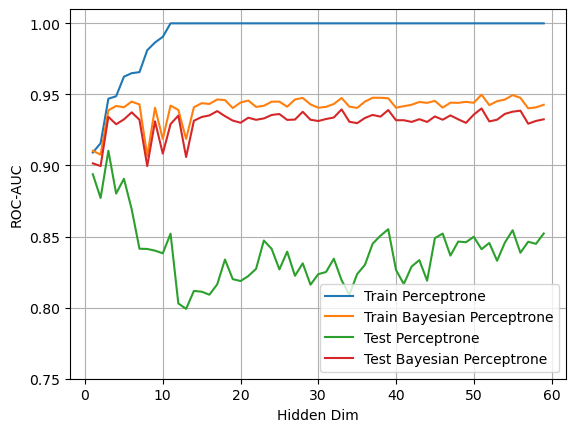
\includegraphics[width=1\linewidth]{roc_auc.png}
        \caption{Зависимость ROC--AUC от размерности скрытого состояния на тренировочных и тестовых данных}
        \label{graph_results}
    \end{figure}
    На рисунке \ref{graph_results} представлены результаты экспериментов.

    \section{Выводы}
    По результатам работы можно сделать следующие выводы:
    \begin{itemize}
        \item с ростом сложности модели байесовская нейронная сеть не переобучилась;
        \item значение ROC-AUC на тестовой выборке
        имеет очень высокую корреляцию со значением ROC-AUC на тренировочной выборке (0.97 по Пирсону).
        Следовательно, для подбора гиперпараметров можно ориентироваться на метрики,
        полученные по тренировочной выборке.
        Это даёт нам возможность отказаться от деления на тренировочную и валидационную выборки
        для подбора гиперпараметров.
    \end{itemize}

    Так же стоит отметить,
    что данный подход переносится на другие архитектуры нейронных сетей
    (рекуррентные, свёрточные, трансформеры).

    Имплементация данного подхода была выполнена с использованием PyTorch.
    Весь исходный код для проведения экспериментов размещён по адресу
    \url{https://github.com/dimabasow/bayesian-neural-networks}.

\end{document}
